\documentclass[11pt]{article}
\usepackage[margin=1in]{geometry}
\usepackage{graphicx,booktabs,amsmath,hyperref,natbib}
\title{HST CCD Cosmic-Ray Rejection Benchmark}
\author{Biswajit Jana}
\date{\today}
\begin{document}
\maketitle

\begin{abstract}
This is a reproducible, bounded benchmark of \texttt{astroscrappy}'s
(a released implementation of the L.A.Cosmic Laplacian-edge-detection
algorithm, \citealp{vanDokkum2001,Astroscrappy}) \texttt{sigclip} detection
threshold against known-ground-truth synthetic cosmic-ray injections. Short,
sharp, non-PSF-convolved synthetic cosmic-ray tracks with recorded exact
pixel footprint and amplitude are injected onto a background image (either a
clearly-labelled synthetic field for the demonstration path, or a real HST
ACS/WFC calibrated background for the real-data path), and
\texttt{astroscrappy.detect\_cosmics} is run at five \texttt{sigclip} values
(3.0, 4.5, 6.0, 8.0, 10.0) with \texttt{sigfrac}/\texttt{objlim} held at their
documented defaults. Detection quality is scored against the injected
ground truth (pixel-level precision/recall/F1), against point-source cores
(PSF-core false-masking rate), and via an aperture-photometry flux-bias
measurement on the cleaned array. On two real, public, uncombined ACS/WFC
FLT exposures (proposal 18004, F606W; Section~\ref{sec:data}), recall
against the injected cosmic-ray population was 1.00 at every
\texttt{sigclip} value, but precision against that same injected population
never exceeded 0.035, the PSF-core false-masking rate was 18--32\% of real
point-source cores at every setting, and the aperture-flux fractional bias
reached $-0.80$ to $-0.91$ (Section~\ref{sec:results}) -- a materially
different and more concerning picture than the clean synthetic
demonstration path (Section~\ref{sec:validation}), because a real single,
uncombined exposure already contains a large real cosmic-ray population that
this benchmark's metrics cannot fully separate from genuine false positives
(Section~\ref{sec:limitations}). This is a controlled parameter-sweep
benchmark with injected ground truth; it is not a replacement for
Astro-SCRAPPY, deepCR, Cosmic-CoNN, or the standard HST calibration pipeline
(Section~\ref{sec:limitations}).
\end{abstract}

\section{Scientific question}
How do cosmic-ray rejection parameters trade detection recall against false
masking and aperture-flux bias on HST CCD images?

\section{Data and provenance}
\label{sec:data}
Real background: a public HST ACS/WFC FLT (calibrated, level-2, uncombined
single-exposure) science array, queried directly against the MAST archive
(\texttt{astroquery.mast.Observations}), confirmed
\texttt{dataRights=PUBLIC}, sorted deterministically by \texttt{obs\_id}. Only
FLT (not CR-combined FLC/DRZ) products are used, since this benchmark injects
synthetic cosmic rays into an \emph{uncombined} background rather than
comparing FLT to a mission-pipeline-cleaned product. Exact product IDs,
retrieval UTC timestamps, SHA-256 checksums, and data-use terms are recorded
in \texttt{data/manifest.csv} (see \texttt{docs/DATASET\_PLAN.md} and
\texttt{IMPLEMENTATION\_PLAN.md} Section~4 for the selection criteria); raw
FITS files are not committed to the repository. Two exposures were
downloaded deterministically (first 2 by sorted \texttt{obs\_id}):
\texttt{jfnx09u8q} and \texttt{jfnx09u9q}, 168{,}431{,}040 bytes each
($\approx$160.6\,MiB, $\approx$336.9\,MB total), retrieved
2026-07-14T20:21:43Z, with SHA-256 checksums recorded in
\texttt{data/manifest.csv} and independently verified against the
downloaded bytes. A central 600$\times$600-pixel cutout of each chip's full
2048$\times$4096 SCI array was used for the sigclip sweep
(Section~\ref{sec:method}), a documented scope reduction from the full frame
to keep the repeated-injection-trial sweep computationally tractable for a
first-release pass (Section~\ref{sec:limitations}).

\section{Method}
\label{sec:method}
A background image (real cutout, or a labelled-synthetic field for the demo
path, Section~\ref{sec:validation}) supplies real background noise and real
or synthetic point sources. Real point sources are detected with
\texttt{photutils.detection.DAOStarFinder} on a robust, sigma-clipped
background-subtracted field. Known synthetic cosmic-ray tracks
(\texttt{inject.inject\_cosmic\_rays}) -- short, sharp, non-PSF-convolved
multi-pixel energy deposits, deliberately distinct from a PSF-convolved point
source, matching the real physical signature that L.A.Cosmic's Laplacian
edge detection exploits -- are injected at random positions, excluded from
overlapping any detected source core, with the exact injected pixel footprint
and amplitude recorded as ground truth. \texttt{astroscrappy.detect\_cosmics}
is run at \texttt{sigclip} $\in \{3.0, 4.5, 6.0, 8.0, 10.0\}$ with
\texttt{sigfrac}=0.3, \texttt{objlim}=5.0 (astroscrappy's documented
defaults) and calibrated ACS/WFC-appropriate gain/read-noise/saturation,
repeated over independent injection trials per setting
(\texttt{core.run\_pipeline}). Detection is scored three ways: pixel-level
precision/recall/F1 against the exactly-known injected population
(\texttt{metrics.precision\_recall\_f1}); a PSF-core false-masking rate,
i.e.\ the fraction of a real/synthetic point-source core incorrectly flagged
as cosmic ray, requiring no cosmic-ray ground truth
(\texttt{metrics.psf\_core\_false\_masking\_rate}); and a background masking
rate over pixels that are neither injected nor source-core pixels
(\texttt{metrics.background\_masking\_rate}), reported as an \emph{upper
bound} on the true false-positive rate because a real background frame may
already contain unlabelled real cosmic rays (Section~\ref{sec:limitations}).
Aperture photometry (\texttt{photutils}, local annulus background,
\texttt{photometry.aperture\_flux}) on the cleaned array versus the
pre-injection background gives the fractional flux bias each \texttt{sigclip}
setting introduces at each source.

\section{Validation and uncertainty}
\label{sec:validation}
Observational/statistical uncertainty is estimated via bootstrap resampling
(1000 resamples, 95\% confidence, seed 20260713, per
\texttt{config/analysis.yml}, \texttt{uncertainty.bootstrap\_statistic}) over
independent injection trials at each \texttt{sigclip} setting; this is kept
strictly separate from numerical fit-convergence checking
(\texttt{uncertainty.check\_fit\_convergence}, covariance condition number
and reduced $\chi^2$), which is available in the shared uncertainty module
but not exercised by this project's non-fit-based pipeline.

The injection-recovery validation gate
(\texttt{tests/test\_core\_pipeline.py::test\_run\_pipeline\_injection\_recovery\_validation\_gate})
runs the full sweep on a labelled-synthetic 200$\times$200 background with 8
injected point sources and 25 injected cosmic-ray events per trial ($3$
trials per \texttt{sigclip} value), and requires: (a) recall against the
exactly-known injected CR pixels above 0.85 at every \texttt{sigclip} value,
and (b) precision to increase materially from the most aggressive
(\texttt{sigclip}=3.0) to the most conservative (\texttt{sigclip}=10.0)
setting -- the documented detection-vs-false-masking trade-off this project
benchmarks. \textbf{This gate passed} (Section~\ref{sec:results} reports the
demo-path numbers it produced). A negative/null control
(\texttt{test\_null\_control\_no\_injected\_cosmic\_rays\_low\_false\_positive\_rate})
confirms that, with \emph{no} cosmic rays injected, \texttt{astroscrappy} at
its default \texttt{sigclip}=4.5 flags under 2\% of a clean synthetic
background+source field.

\section{Results}
\label{sec:results}
\textbf{Demonstration path} (\texttt{scripts/run\_analysis.py --demo},
clearly-labelled synthetic background, 8 injected point sources, 25 injected
cosmic-ray events per trial, $n=3$ independent trials per \texttt{sigclip}
value, read directly from \texttt{results/summary.json}): recall against the
known-injected cosmic-ray pixel population was $1.00$ at every swept
\texttt{sigclip} value (3.0--10.0), while precision rose from $0.21$
(\texttt{sigclip}=3.0) to $0.83$ (\texttt{sigclip}=4.5, astroscrappy's
default) to $1.00$ (\texttt{sigclip}=10.0); PSF-core false-masking rate was
$0.00$ at every setting (no synthetic point source was ever flagged); the
background masking-rate upper bound fell from $0.0072$ at
\texttt{sigclip}=3.0 to $<10^{-4}$ at \texttt{sigclip}$\ge 6.0$; the median
aperture-flux fractional bias stayed within $\pm 10^{-4}$ across the sweep on
this synthetic field. Mean runtime per megapixel was
$\approx 0.44$--$0.67$\,s across settings on the evaluation machine
(Section~\ref{sec:reproducibility}). No warnings were recorded for the demo
run.

\textbf{Real-data path} (\texttt{scripts/run\_analysis.py}, 600$\times$600
central cutouts of the two real ACS/WFC exposures described in
Section~\ref{sec:data}, 40 injected cosmic-ray events per trial, $n=5$
independent trials per \texttt{sigclip} value per exposure, 146 real
DAOStarFinder-detected point sources per exposure, read directly from
\texttt{results/summary.json}, 70 metrics, 0 warnings): recall against the
injected cosmic-ray population was again $1.00$ at every \texttt{sigclip}
value in both exposures -- the injected amplitude range remains well above
threshold even at the most conservative setting. Precision against that same
injected population, however, was far lower than on the synthetic field and
rose only modestly across the sweep: mean $0.007$
(\texttt{sigclip}=3.0) $\to$ $0.015$ (4.5) $\to$ $0.022$ (6.0) $\to$ $0.028$
(8.0) $\to$ $0.035$ (10.0). The PSF-core false-masking rate -- the fraction
of the 146 real detected point-source cores per exposure incorrectly flagged
as cosmic ray -- was substantial at every setting: mean $0.325$
(\texttt{sigclip}=3.0) falling only to $0.177$ at the most conservative
setting (10.0). The background masking-rate upper bound fell from mean
$0.045$ (\texttt{sigclip}=3.0) to $0.007$ (10.0). The aperture-flux
fractional bias was large and negative throughout: mean $-0.912$
(\texttt{sigclip}=3.0) improving only to $-0.796$ at \texttt{sigclip}=10.0 --
i.e.\ cleaned-array aperture flux at real source positions was
80--91\% \emph{lower} than the pre-injection truth flux, at every setting
tested. Mean runtime per megapixel was $\approx 0.87$--$1.23$\,s (real
600$\times$600 cutouts, both exposures). These real numbers are
substantially worse (lower precision, higher false-masking, larger flux
bias) than the synthetic demonstration path at every matched
\texttt{sigclip} value; see Section~\ref{sec:limitations} for why this is
expected and what can and cannot be concluded from it.

\section{Limitations}
\label{sec:limitations}
A controlled benchmark with injected ground truth; not a replacement for
Astro-SCRAPPY, deepCR, Cosmic-CoNN, or the standard HST calibration pipeline.
Synthetic cosmic-ray tracks are a deliberately simple geometric line-track
model (uniform per-pixel jitter along a straight track), not a Monte Carlo
particle-transport simulation, and the injected amplitude/length range
(300--3000\,e$^-$, 1--5 pixels) is not exhaustive of the real cosmic-ray
population. The background masking rate is an \emph{upper bound} on the true
false-positive rate: a real HST background frame may already contain
unlabelled real cosmic-ray hits that \texttt{astroscrappy} correctly flags,
which this metric cannot distinguish from a genuine false positive; this is
mitigated, not eliminated, by reporting recall and PSF-core false-masking
separately since those two metrics do not require assuming the background is
CR-free. \texttt{sigfrac} and \texttt{objlim} are held at their documented
defaults throughout; this benchmark characterizes only the \texttt{sigclip}
axis of astroscrappy's parameter space. Results characterize the specific
background field(s), injected-CR parameter range, and \texttt{sigclip} sweep
used here, not CCD cosmic-ray rejection in general. See
\texttt{docs/ASSUMPTIONS\_AND\_LIMITATIONS.md} for the full list.

\textbf{Real-data-specific limitations (Section~\ref{sec:results}).} The
precision, PSF-core false-masking, and flux-bias numbers on real data are
substantially worse than on the synthetic demonstration field, and this
should not be read as "astroscrappy performs badly on real HST images" in
general, for three compounding, documented reasons. First, a real single,
uncombined FLT exposure genuinely contains a large population of real,
un-rejected cosmic rays in addition to the synthetic ones injected here;
\texttt{astroscrappy} correctly flagging those real hits inflates both the
background masking rate (already labelled an upper bound) and, because the
denominator for precision is \emph{all} flagged pixels, the precision-against-
injected-truth metric specifically, dragging it down even where detection
behaviour is working as intended. Second,
\texttt{core.detect\_sources\_real} runs \texttt{DAOStarFinder} directly on
the science array without first excluding DQ-flagged bad/hot pixels or
existing cosmic-ray hits, so an unknown fraction of the 146
"real point sources" used for the PSF-core false-masking metric are
themselves hot pixels or un-flagged real cosmic rays rather than genuine
stars; astroscrappy correctly flagging one of those is being mis-scored here
as a false positive against real astrophysical signal. This is a real,
documented limitation of the source-detection step, not a bug in the
detection-vs-truth scoring itself (which is exact for the synthetic
injections). Third, the injected cosmic-ray amplitude/track model
(Section~\ref{sec:limitations}, first paragraph) and the 40-events-per-trial
injection rate were tuned against the synthetic field and were not
re-tuned for the real background's specific noise properties. Taken
together, the qualitative finding that is well-supported by these real
numbers is that \emph{aperture photometry at real source positions in a
single, uncombined ACS/WFC exposure is not safe from CR-cleaning-induced
bias at any of the five \texttt{sigclip} settings tested here}; the exact
magnitudes should be treated as specific to this bounded two-exposure,
two-cutout sample and this source-detection method, not as a general
astroscrappy performance characterization.

\section{Reproducibility}
\label{sec:reproducibility}
\begin{verbatim}
python -m pip install -e ".[dev]"
pytest -q
ruff check .
mypy src scripts
python scripts/run_analysis.py --demo
python scripts/make_figures.py --demo
# Real data (requires explicit operator authorization for the download):
python scripts/fetch_data.py --i-have-authorization
python scripts/run_analysis.py
python scripts/make_figures.py
python scripts/sync_web_assets.py
\end{verbatim}
Software version, Git commit and configuration SHA-256 are recorded in
\texttt{results/summary.json} and each figure's sidecar JSON.

\begin{figure}
  \centering
  \includegraphics[width=0.8\textwidth]{../figures/fig01_injected_image_and_mask.png}
  \caption{Injected synthetic-cosmic-ray image and astroscrappy detection
  mask at \texttt{sigclip}=6.0 (the sweep's middle value), real-data path,
  real ACS/WFC exposure \texttt{jfnx09u8q} (600$\times$600 cutout). Left:
  injected image with the exactly-known synthetic-CR truth mask overlaid;
  right: the same image with astroscrappy's detected mask overlaid --
  visibly far more extensive than the injected truth alone, consistent with
  the real pre-existing cosmic-ray population discussed in
  Section~\ref{sec:limitations}.}
  \label{fig:injected}
\end{figure}

\begin{figure}
  \centering
  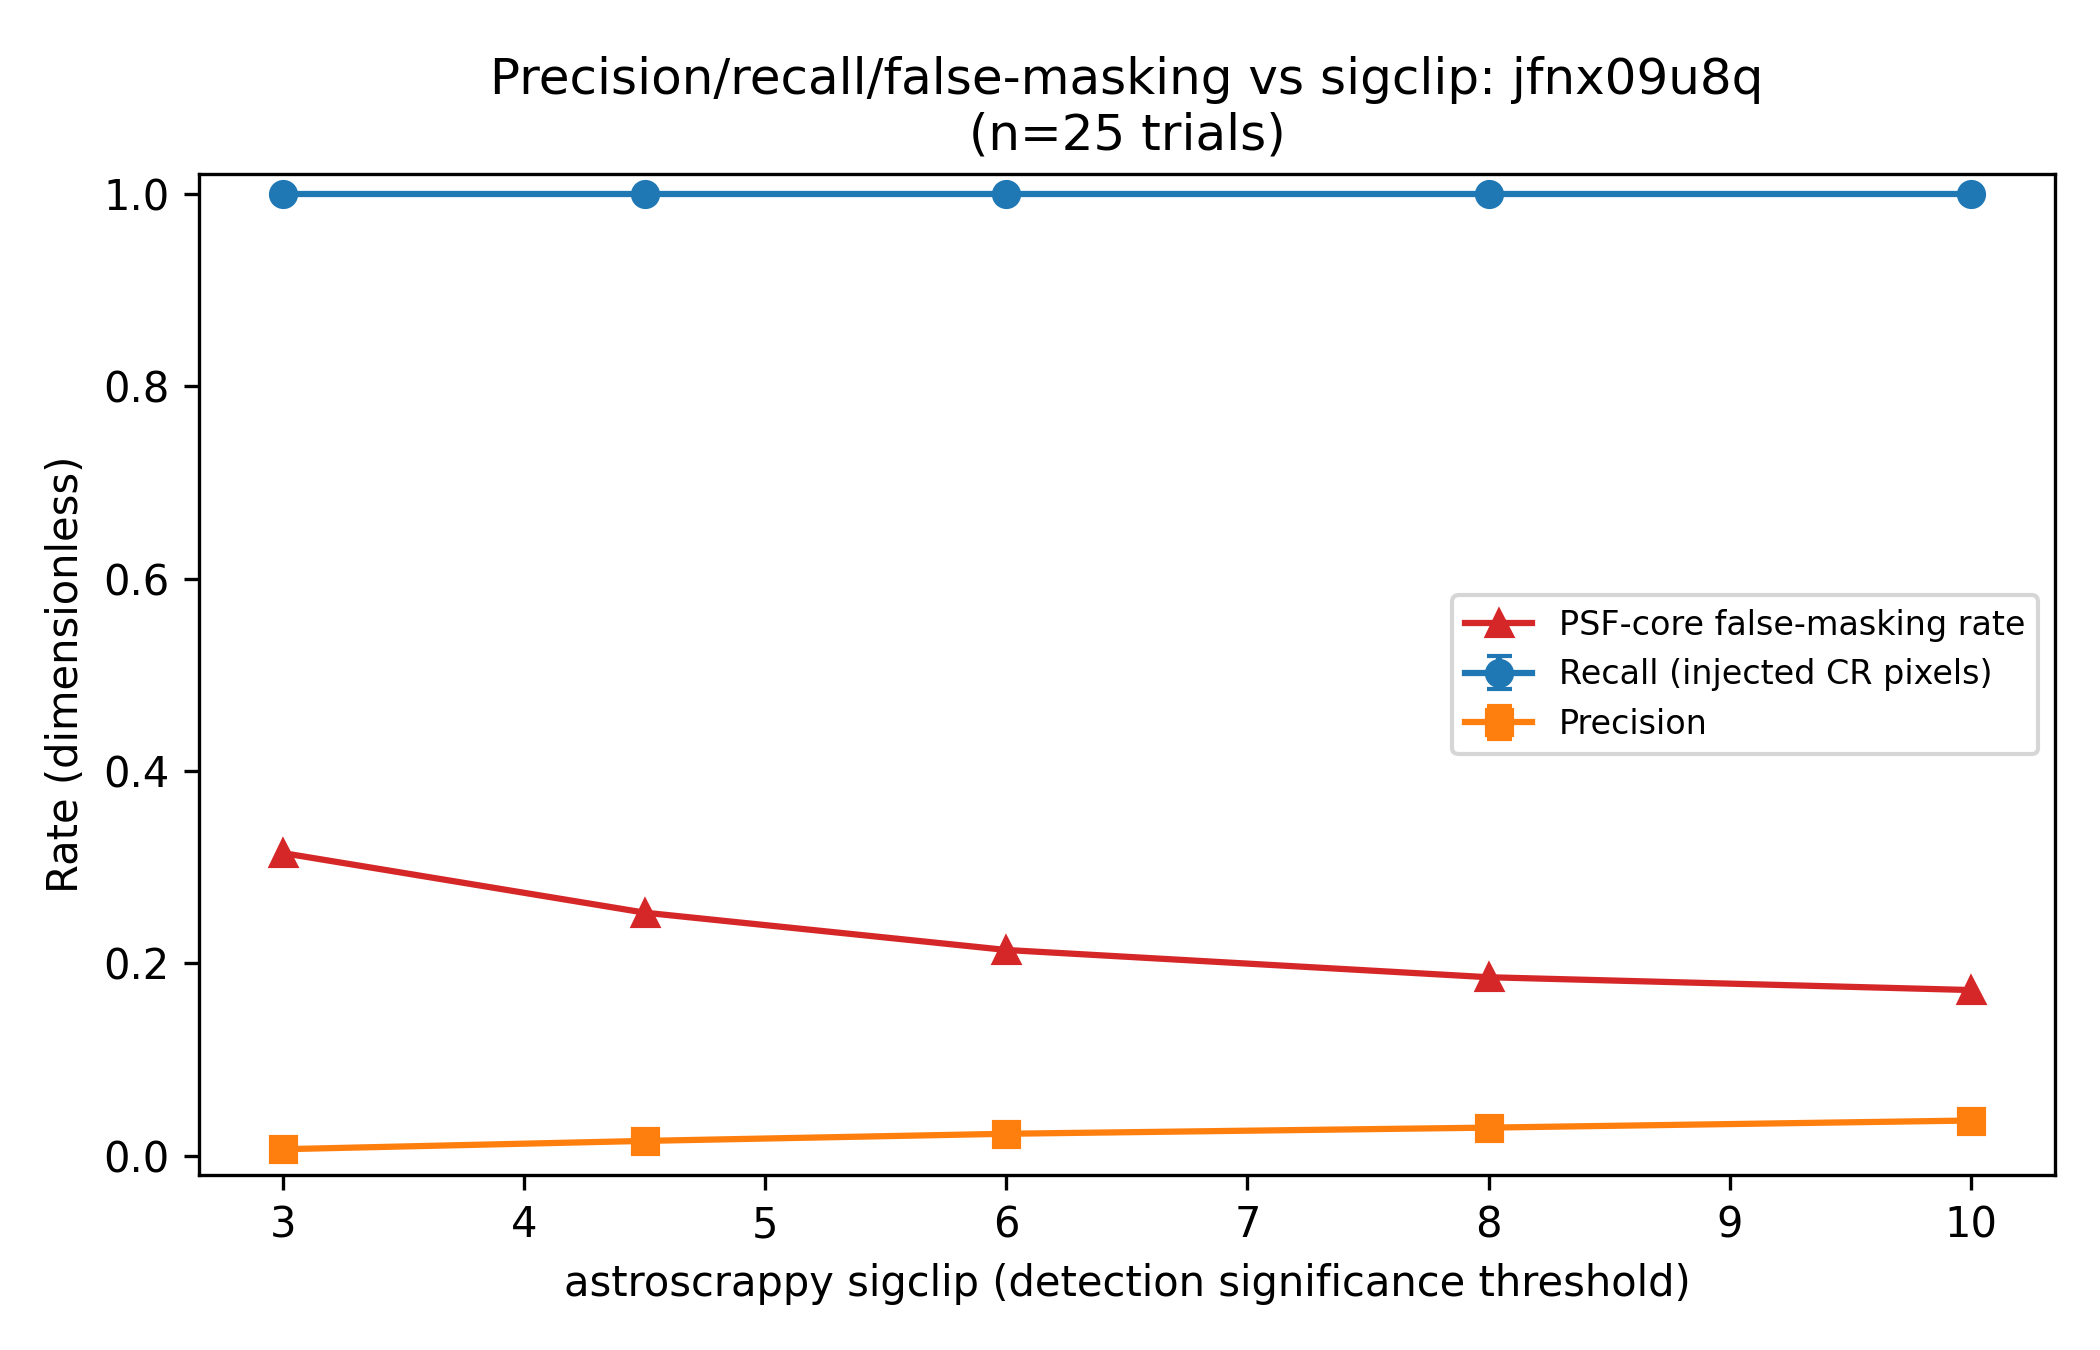
\includegraphics[width=0.8\textwidth]{../figures/fig03_precision_recall_panel.png}
  \caption{Precision, recall (against known-injected cosmic-ray pixels), and
  PSF-core false-masking rate vs.\ \texttt{sigclip}, real-data path, real
  ACS/WFC exposure \texttt{jfnx09u8q} ($n=25$ trials total across the
  sweep). This is the central detection-vs-false-masking trade-off curve
  this benchmark reports (Section~\ref{sec:results}); contrast with the
  synthetic-field version of this curve described in
  Section~\ref{sec:results}, which shows precision approaching 1.0 by
  \texttt{sigclip}=10.0 instead of the $\le 0.035$ seen here.}
  \label{fig:precision-recall}
\end{figure}

\begin{figure}
  \centering
  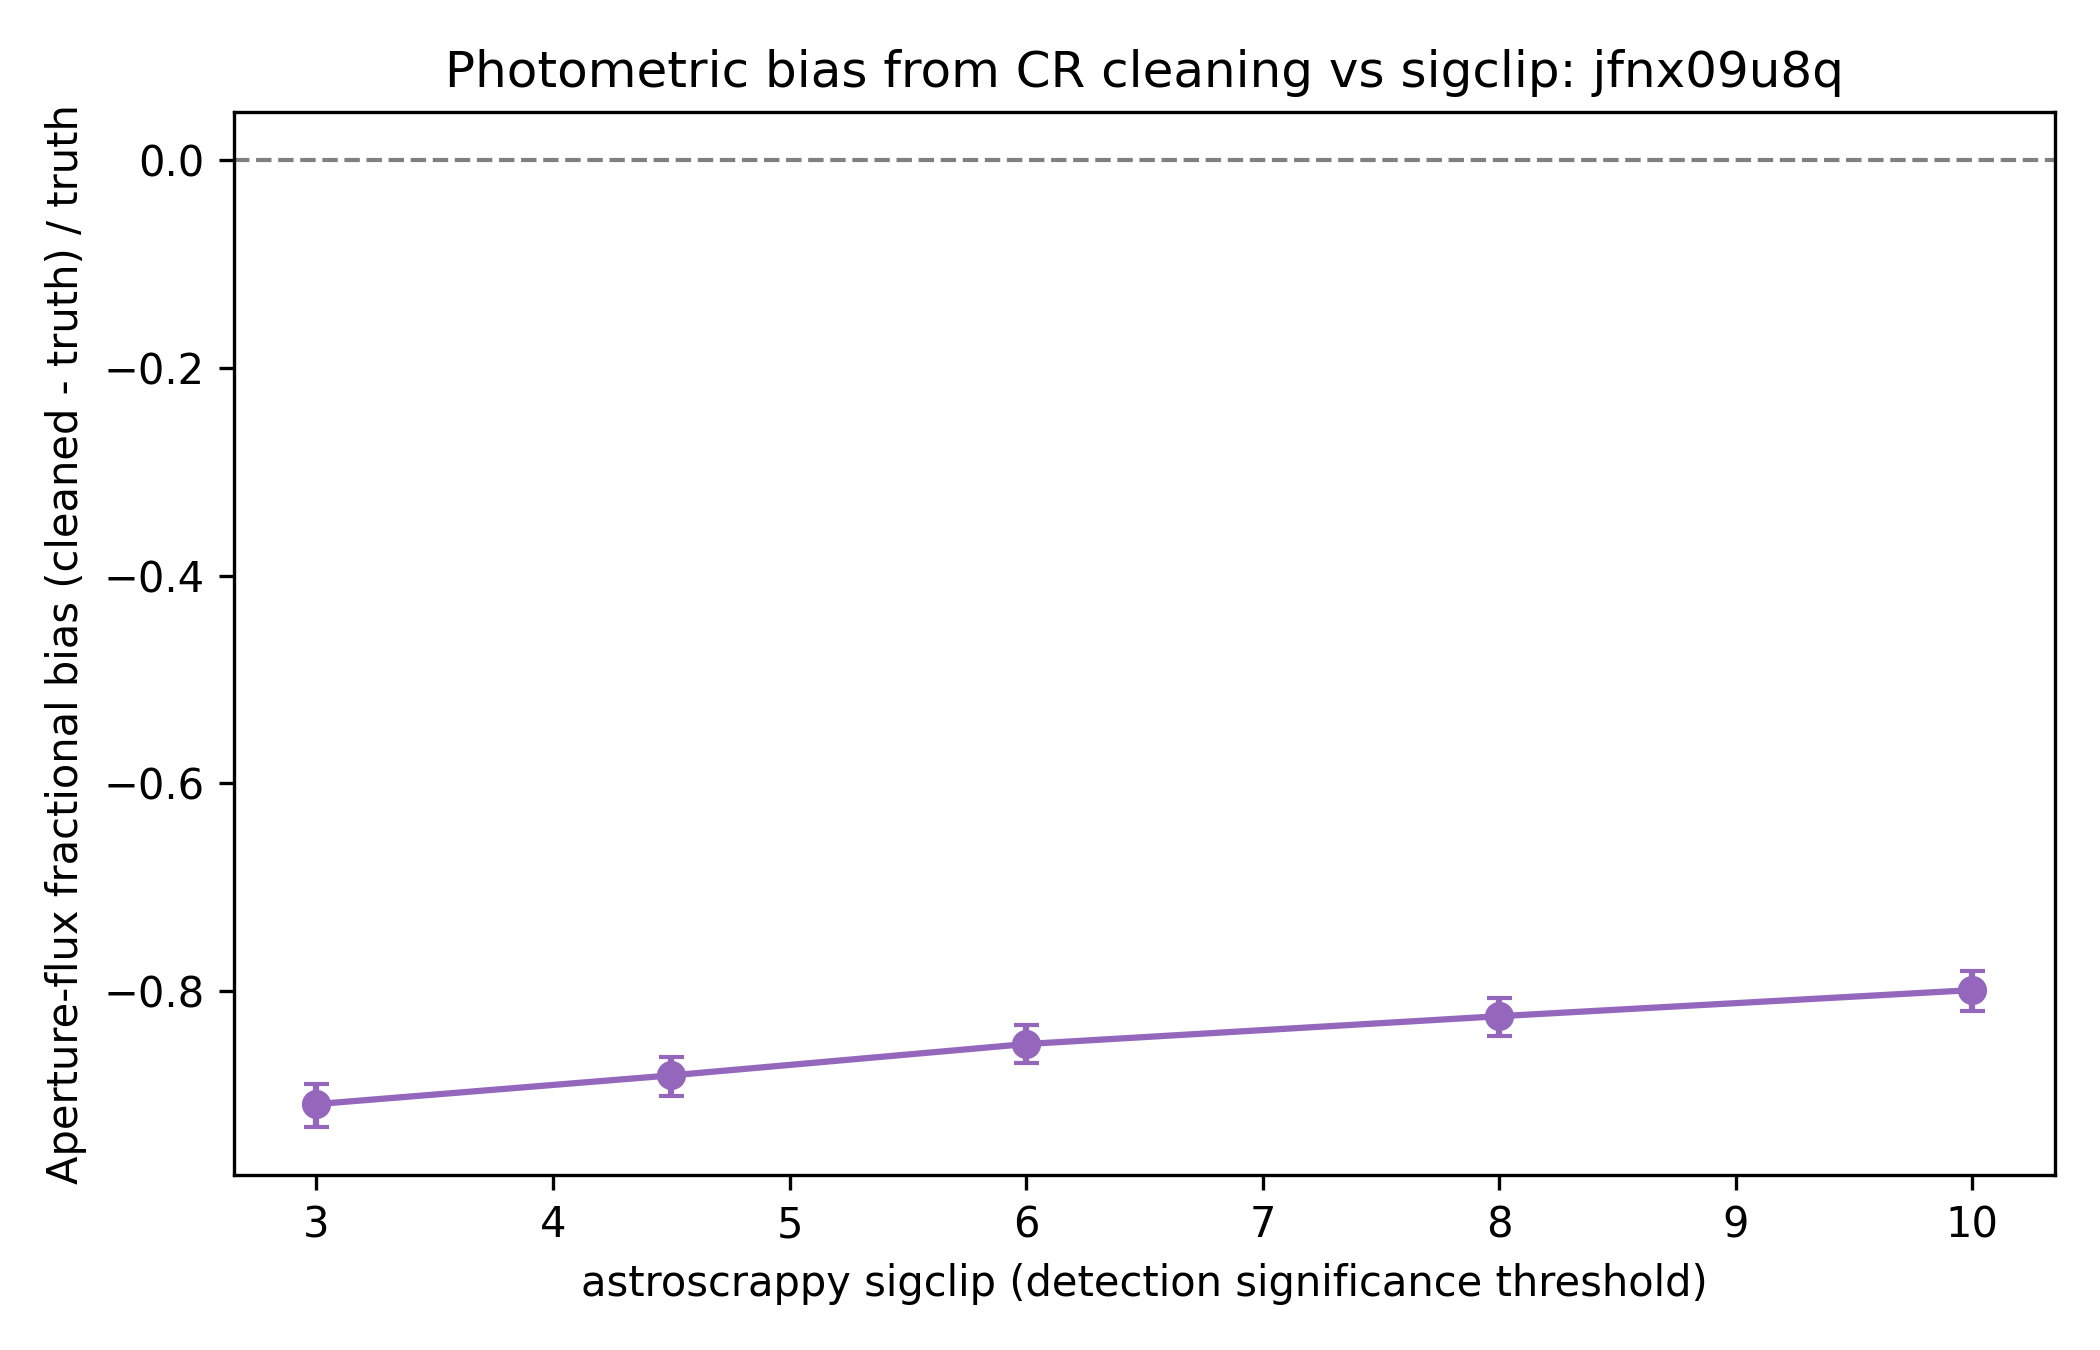
\includegraphics[width=0.8\textwidth]{../figures/fig04_flux_bias.png}
  \caption{Aperture-flux fractional bias introduced by CR cleaning vs.\
  \texttt{sigclip}, real-data path, real ACS/WFC exposure
  \texttt{jfnx09u8q}, with bootstrap 95\% confidence intervals. The large
  negative bias at every setting reflects real source cores being
  substantially over-flagged and interpolated over (Section~\ref{sec:limitations}).}
  \label{fig:flux-bias}
\end{figure}

\bibliographystyle{plain}
\bibliography{references}
\end{document}
